\section{Proposed Methodology}\label{sec:4_first_proposed_approach}

In this section, we present the primary phases of our study, comprising three distinct stages. Following this introduction, we delve into the synthetic data-generator method, providing a comprehensive breakdown of the four essential steps. Our proposal aims to develop a robust approach designed to overcome the challenging domain of multiclass classification for imbalanced and drifting data streams. In pursuit of this goal, our proposal addresses the four primary challenges inherent in constructing our approach.
\begin{itemize}
	\item \textbf{Multiclass Imbalanced Streams:} This study focuses on addressing the widespread problem of imbalanced data streams in the context of multiple classes. We aim to address this issue using well-known techniques, notably MLSMOTE and MLSOL.
	\item \textbf{Class Overlap:} We also address a critical challenge involving class overlapping, a factor known to substantially affect model performance [23] [24]. To address this issue, we introduce an adaptive method that generates nonoverlapping synthetic instances, thereby enhancing the overall performance of the model.
	\item \textbf{Drifted Streams:} Our proposed approach integrates a concept drift detector to identify shifts in the underlying data distribution. This dynamic detection mechanism enables the model to promptly recognize changes and adjust its classifiers, thereby ensuring its effectiveness in handling drifting stream.
	\item \textbf{Classifier Performance:} To enhance the classifier performance, our approach employs Dynamic Ensemble Selection (DES). This technique creates a pool of classifiers and dynamically selects the most suitable classifier for each incoming data point, further improving classification accuracy and robustness.
\end{itemize}

\subsection{Approach Overall Details}

Our proposed approach is designed with three distinct phases that work together to improve its performance in managing multiclass imbalanced and drifting data streams. 
\begin{itemize}
	\item \textbf{DES Phase (dynamic ensemble selection phase):} The first phase, known as the dynamic ensemble selection (DES) phase, is responsible for selecting the most appropriate classifier for the incoming data. This ensures that the selected classifier is well-suited for the current data chunk.
	\item \textbf{Drift detector phase:} The second phase of our approach is the drift detector phase, which operates in real-time to continuously monitor the data stream. Its primary function is to identify any signs of concept drift, which indicates shifts in the underlying data distribution over time.
	\item \textbf{Synthetic data generator phase:} The final phase of our approach is the synthetic data generator phase, which is dedicated to generating synthetic data for the minority classes. This step is crucial for addressing class imbalance by producing additional samples for underrepresented classes, thereby significantly enhancing the model's ability to accurately classify instances from minority classes.
\end{itemize}

Specifically, as shown in Fig. \ref{fig:4_first_proposal_step_1}, the DES phase retrieves the current data chunk from the stream and applies the DES technique to select the most suitable classifiers for the received chunk. The selected classifiers were then passed to the second phase, where they were employed to predict the class of each instance within the received data chunk. Simultaneously, detectors like ADWIND or DDM are employed to monitor any occurrence of concept drift. If the discrepancy between the class frequency and standard deviation of the current chunk is significant, as described in reference [37], and the imbalance ratio exceeds the average imbalance ratio, the current chunk is forwarded to the third phase, as indicated by the red rectangle in Fig. 1. In the third phase, our proposed method uses a set of equations 	\ref{eq:4_first_proposal_1}\ref{eq:4_first_proposal_2}\ref{eq:4_first_proposal_3}
to identify minority classes. The first equation calculated the frequency of each class in the current chunk. The second equation determines the optimal frequency for each class based on the size of the chunk and the number of classes in the current chunk. Finally, the third equation designates the classes as minority classes if their frequency differs significantly from the standard deviation of the current chunk.
As shown in Fig. \ref{fig:4_first_proposal_step_2}, phase These identified minority classes are then fed into the synthetic data generator phase, which increases the minority class samples to balance any imbalanced chunks. This ensures optimal performance for the new classifiers. Algorithm  \ref{alg:4_first_proposal_2} provides a comprehensive outline of the process of the proposed approach, which is the main contribution of our study and is designed to effectively address multiclass imbalanced and drifting data streams, uses streaming data as input, and systematically executes each step within the approach. The outcome of this process is the classification prediction generated using the proposed approach.


\subsection{Synthetic Data Generator}

Fig. \ref{fig:4_first_proposal_step_2} presents a comprehensive overview of the synthetic data generator phase, which is an essential component responsible for generating synthetic samples by considering both data distribution and historical chunk behaviors. This phase has several advantages and can perform a wide range of tasks.
\begin{itemize}
	\item \textbf{Similar chunk analysis:} Initially, the phase analyzes the current chunk distribution and identifies a similar chunk from historical data. This analysis forms the basis for generating synthetic samples that align with prevailing distribution patterns.
	\item \textbf{Oversampling method selection:} This phase utilizes the knowledge of the oversampling technique applied to the identified similar chunk. Consequently, it employs an alternative oversampling technique, using MLSMOTE and MLSOL, to create the most effective synthetic data. This step is designed not only to optimize the current classification but also to preemptively address potential drifts in similar future chunks.
	\item \textbf{Class overlap validation:} This step involves generating synthetic samples for the minority classes to effectively address the issue of minority classes and consequently enhance the classifier performance. The process utilizes the K-Nearest Neighbor (KNN) algorithm, as applied in [25], to identify overlaps between newly generated data instances and existing instances. If overlaps are detected, the proposed approach iteratively removes these samples because their presence can potentially diminish the overall classifier performance [23] [24]. Consequently, the proposed approach generates alternative samples to address this challenge and preserve the primary objectives of the synthetic data generator step.
	\item \textbf{Continuous refinement:} This process iterates until it successfully generates high-quality synthetic data that aligns with the data distribution, minimizes overlap, and mitigates potential concept drift. The generated data were subsequently utilized in the training phase to improve classifier accuracy.
\end{itemize}

In Algorithm \ref{alg:4_first_proposal_2}, also known as the Synthetic Data Generator, we input three essential elements: the minority class samples, the current data chunk, and the desired size for generating synthetic data. The primary objective of this algorithm is to produce synthetic data samples. To achieve this, we employ the KNN algorithm to identify any overlapping instances within the current chunk (Line 3). This algorithm utilizes two specific techniques, MLSMOTE  [37] and MLSOL [33]. MLSMOTE was chosen for its introduction of randomness during instance generation, reducing its reliance on the local characteristics and distribution of the minority class. This randomization diminishes the likelihood of producing overlapping instances, particularly in cases where minority class instances are situated in overlapping regions. In contrast, MLSOL considers the local behavior of minority classes, resulting in synthetic points that closely resemble the minority class. This approach significantly improves the accuracy of the classifier (lines 4-10). Additionally, in this algorithm, specifically from lines 11 to 17, these lines are dedicated to generating synthetic instances that ensure non-overlap with existing classes. This procedure depends on the selected oversampling method and utilizes the KNN algorithm to guarantee that the generated instances do not overlap with the existing ones.
\begin{figure}[!ht]
	\centering
	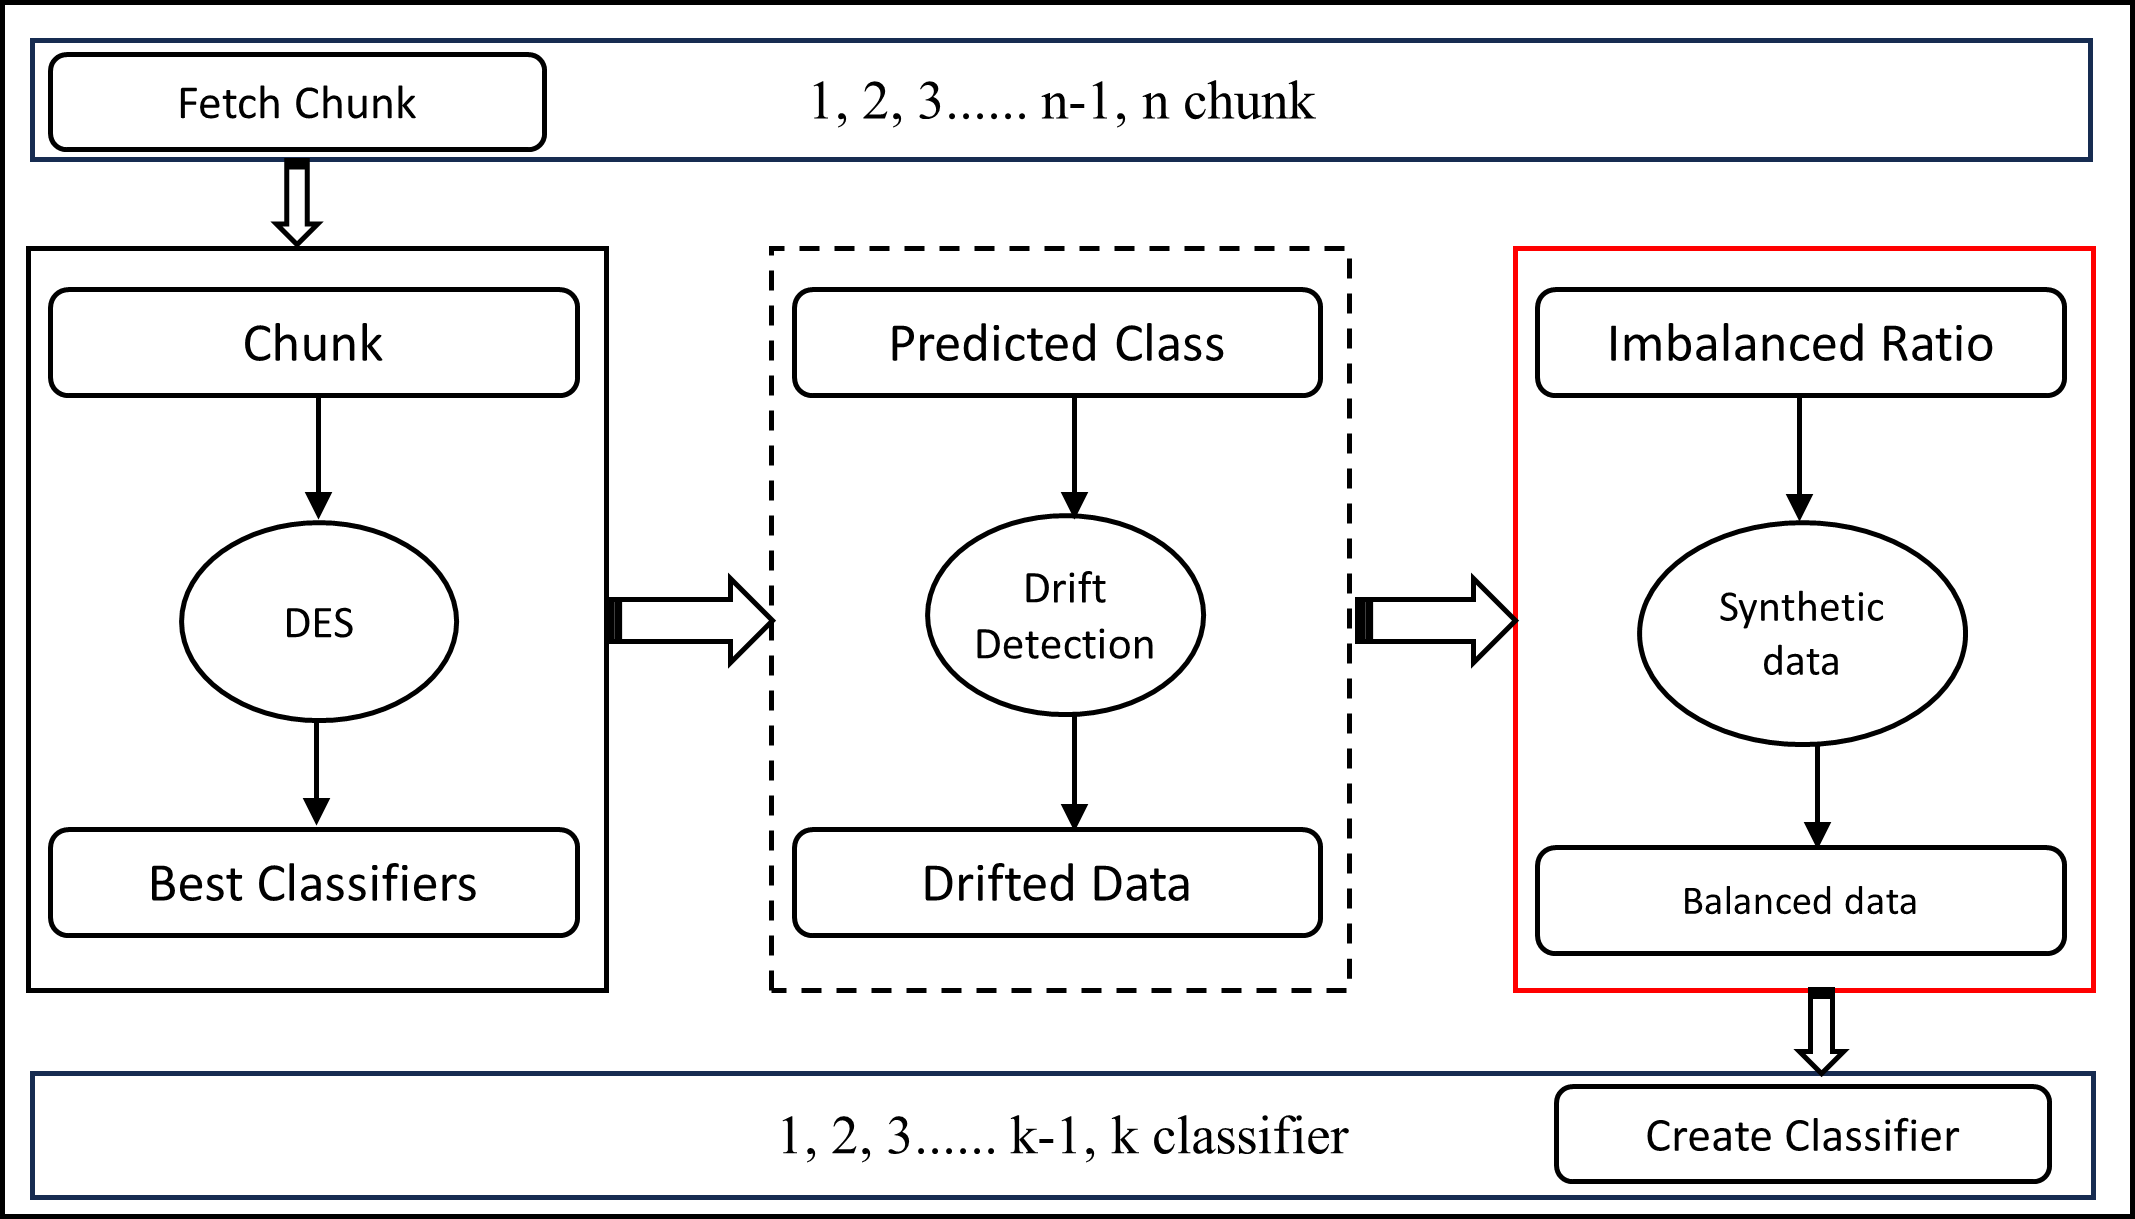
\includegraphics[width=1\linewidth]{4_Taxonomy/figures/approach_step_1.png}
	\caption{Proposed Approch Flow.}
	\label{fig:4_first_proposal_step_1}
\end{figure}
\begin{figure}[!ht]
	\centering
	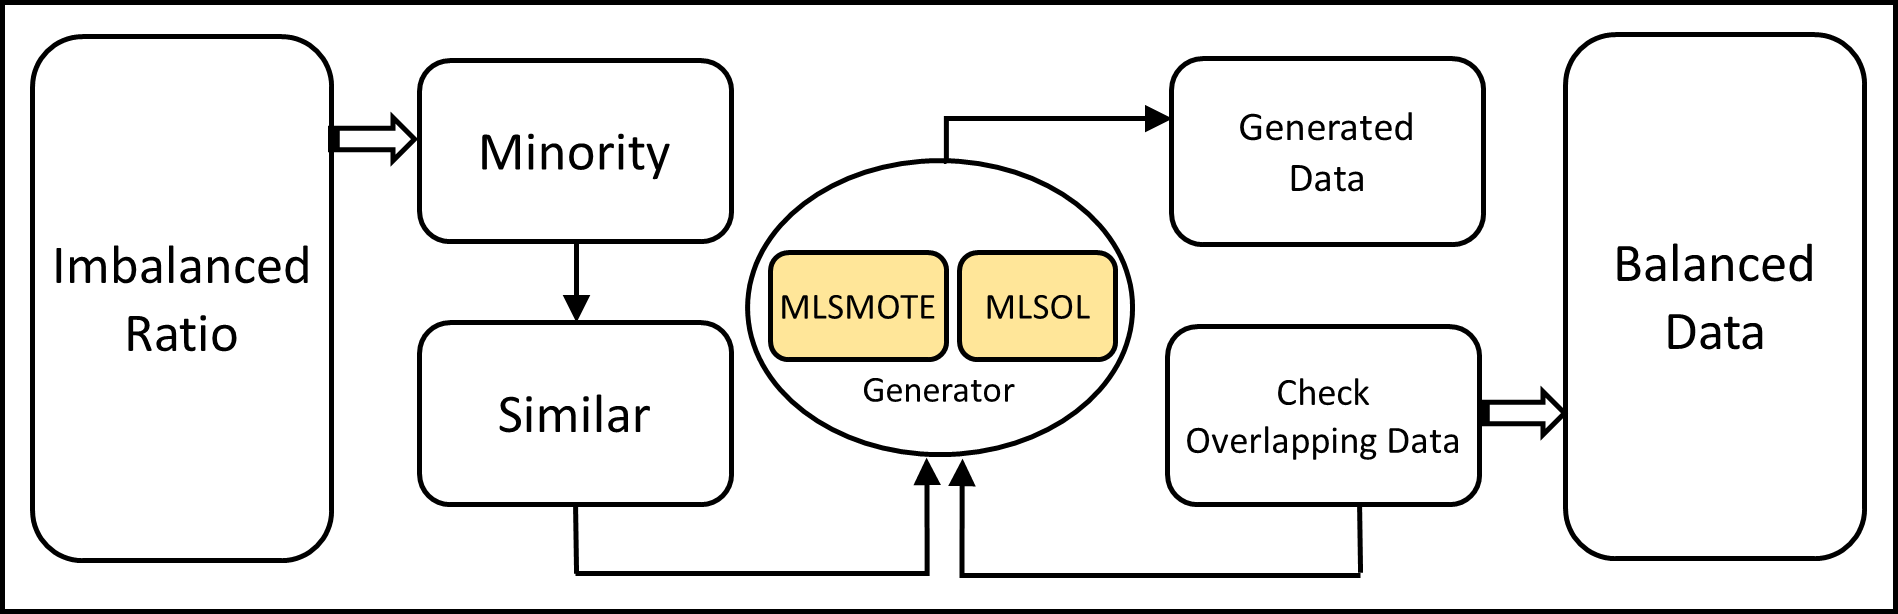
\includegraphics[width=1\linewidth]{4_Taxonomy/figures/approach_step_2.png}
	\caption{Synthetic Data Generator Flow.}
	\label{fig:4_first_proposal_step_2}
\end{figure}

\begin{equation}
	\label{eq:4_first_proposal_1}
    frq_{c} = \sum_{i=1}^{\text{chunk size}} \begin{cases} 
    1, & \text{if } y_i = c \\
    0, & \text{otherwise}
    \end{cases}, \quad i = 1, 2, 3, \dots \text{chunk size}\;
\end{equation}

\begin{equation}
	\label{eq:4_first_proposal_2}
    \text{best } freq_{n} = \frac{|n|}{|C|}
\end{equation}

\begin{equation}
	\label{eq:4_first_proposal_3}
    \text{classes type}_{\text{chunk}} = \sum_{c=1}^{C} \begin{cases} 
    \text{Minority,} & \text{if } diff(sd_c - frq_i) > \text{best } freq_{\text{chunk}} \\
    \text{Majority,} & \text{otherwise}
    \end{cases}, \quad c = 1, 2, 3, \dots C
\end{equation}


\begin{algorithm}[H]
\caption{Proposed Framework Algorithm for Imbalanced Multi-Class Drifted Data Streams}
\KwIn{data stream, maximum classifiers pool size $\kappa$}
% \Parameter{current chunk $a$, synthetic data $b$, classifiers pool $\Psi$, drifted pool $\psi$, classes frequency $\Omega$, best frequency $\omega$, minority classes $\mu$}
\KwOut{Prediction $P$}
\BlankLine
$\psi, \Psi, \Omega, \mu \gets \emptyset$\;
$\omega \gets 0$\;
\For{stream have chunk}{
    \eIf{$a$ is the First chunk}{
        $k \gets$ \texttt{trainingNewClassifier}($a$)\;
        $P \gets$ \texttt{getPrediction}($a, k$)\;
    }{
        $k \gets$ \texttt{DES}($a, \Psi$)\;
        $P \gets$ \texttt{getPrediction}($a, k$)\;
        $\psi \gets$ \texttt{conceptDriftDetector}($P$)\;
        \If{$\psi > 0$}{
            $\Omega \gets$ get classes frequency according to Eq.1\;
            $\omega \gets$ best frequency according to Eq.2\;
            $\mu \gets$ get minority classes according to Eq.3\;
            $b \gets$ utilize $a$ and $\mu$ to get the synthetic data according to Algorithm 2\;
            trainingData $\gets a + b$\;
            $k \gets$ \texttt{trainingNewClassifier}(trainingData)\;
            $\Psi \gets \Psi + k$\;
            \If{$\Psi > \kappa$}{
                \texttt{removeWorstClassifier}($\Omega$)\;
            }
        }
        $P \gets$ \texttt{getPrediction}($a, k$)\;
    }
}
\Return{$P$}
\end{algorithm}
\begin{algorithm}[H]
	\caption{Synthetic data generator}
	\KwIn{Minority classes $\mu$, current chunk $a$, sample size $\eta$, historical chunks $h$}
	\KwOut{Generated data $b$}
	$b \gets \emptyset$\;
	$f \gets \text{MLSMSOTE}$\;
	$knn \gets \text{kNearestNeighbor}(a)$\;
	$chunk \gets \text{similarChunk}(a, h)$\;
	$f \gets \text{similarChunkOverSamplingMethod}(chunk)$\;
	\If{$f = \text{MLSMSOTE}$}{
		$f \gets \text{MLSOL}$\;
	}
	\Else{
		$f \gets \text{MLSMSOTE}$\;
	}
	\While{$|b| < \eta$}{
		$p \gets \text{generateSyntheticPoint}(\mu, f)$\;
		$similarPointsClass \gets \text{KNN.getKneighbor}(b)$\;
		\If{$similarPointsClass = \mu$}{
			$b \gets b \cup \{p\}$\;
		}
	}
	\Return $b$\;
	\end{algorithm}